 \chapter{Implementación de los módulos}

El presente capítulo describe la implementación de cada módulo del sistema de navegación
asistida, detallando su diseño interno, sus entradas y salidas, los algoritmos empleados
y su pseudocódigo correspondiente. La organización sigue la arquitectura modular definida
en el marco metodológico y justificada en el análisis de requerimientos, cubriendo los
cuatro grupos de módulos: percepción, representación, navegación y rutas, e interacción.

Las tecnologías asignadas a cada módulo y los requerimientos que motivan cada elección
se resumen en la Tabla~\ref{tabla_tecnologias} del capítulo anterior.

% ==========
\section{Módulos de percepción}
% ===========

Los módulos de percepción transforman las señales físicas del entorno, fotogramas de
cámara y lecturas de sensores de proximidad en información estructurada que los módulos
de representación y navegación pueden procesar. Su flujo interno se ilustró en la
Figura~\ref{fig:flujo_vision}.


% ------------------------------------------------------------------------------
\subsection{Procesamiento de imágenes}
% ------------------------------------------------------------------------------

\textbf{Descripción:}
Este módulo prepara cada fotograma capturado por la cámara para que pueda ser procesado
de forma eficiente y estable por el módulo de visión. Su objetivo es reducir la
variabilidad innecesaria en la imagen, estandarizar las condiciones de entrada y eliminar
artefactos visuales que puedan afectar la detección.

\textbf{Entradas:}
\begin{itemize}
    \item Fotograma capturado por la cámara (imagen en bruto)
\end{itemize}

\textbf{Salidas:}
\begin{itemize}
    \item Imagen preprocesada lista para el módulo de visión
\end{itemize}

\textbf{Procesos realizados:}
\begin{itemize}
    \item Redimensionamiento al tamaño de entrada requerido por el modelo de visión
    \item Normalización de valores de píxel al rango $[0, 1]$
    \item Igualación de histograma para compensar variaciones de iluminación
    \item Filtrado gaussiano para reducción de ruido de alta frecuencia
\end{itemize}

\textbf{Tecnologías utilizadas:} OpenCV, NumPy

Se puede encontrar el pseudocódigo utilizado para el procesamiento de imágenes en el apéndice \ref{apend:procesa}

% ------------------------------------------------------------------------------
\subsection{Módulo de visión}
% ------------------------------------------------------------------------------

\textbf{Descripción:}
Este módulo aplica un modelo de detección de objetos sobre la imagen preprocesada para identificar los elementos relevantes del entorno en tiempo real. Por cada objeto detectado genera una región de interés (bounding box), su categoría semántica y un nivel de confianza. Además, asigna a cada objeto un nivel de riesgo para la navegación, distinguiendo entre elementos de riesgo inmediato y elementos que forman parte del entorno
navegable sin representar una amenaza.

\textbf{Entradas:}
\begin{itemize}
    \item Imagen preprocesada (proveniente del módulo de procesamiento de imágenes)
\end{itemize}

\textbf{Salidas:}
\begin{itemize}
    \item Lista de objetos detectados, cada uno con:
    \begin{itemize}
        \item Clase semántica (persona, puerta, escalera, obstáculo, pared, etc.)
        \item Región de interés (coordenadas de la caja delimitadora)
        \item Nivel de confianza de la detección (valor entre 0 y 1)
        \item Nivel de riesgo asignado (alto, medio, bajo)
    \end{itemize}
\end{itemize}

\textbf{Modelo empleado:} YOLOv8 (Ultralytics). Se elige por su arquitectura de una sola etapa, que realiza extracción de características y predicción de objetos en un único
paso, lo que permite cumplir la restricción de latencia de 300~ms establecida en RNF-01.

\textbf{Tabla de niveles de riesgo:}

\begin{table}[H]
\centering
\begin{tabular}{ll}
\hline
\textbf{Clase de objeto} & \textbf{Nivel de riesgo} \\
\hline
Persona (en movimiento) & Alto \\
Escalera / desnivel     & Alto \\
Obstáculo estático      & Medio \\
Puerta (cerrada)        & Medio \\
Puerta (abierta)        & Bajo \\
Pared / superficie      & Bajo \\
\hline
\end{tabular}
\caption{Clasificación de riesgo por tipo de objeto detectado}
\label{tabla_riesgo}
\end{table}

\subsubsection{Pseudocódigo del módulo de visión}

\begin{center}
\captionof{algorithm}{Pseudocódigo del módulo de visión}
\label{alg:vision}
\end{center}
\vspace{-1.8cm}
\rule{\textwidth}{0.4pt}
\vspace{-0.9cm}

\begin{algorithmic}[1]

\Statex \textbf{ENTRADA:}
\Statex imagen\_lista
\Comment{imagen preprocesada}

\Statex
\Statex \textbf{SALIDA:}
\Statex lista\_detecciones
\Comment{lista de objetos con clase, caja, confianza y riesgo}

\Statex
\State Ejecutar el modelo de detección sobre la imagen

\State resultados\_brutos $\gets$
modelo\_deteccion.inferir(imagen\_lista)

\Statex
\Statex \textbf{PROCESO}
\State Filtrar resultados por umbral mínimo de confianza (umbral = 0.5)

\State lista\_detecciones $\gets$ []

\Statex

\For{cada resultado EN resultados\_brutos}

    \If{resultado.confianza >= umbral\_confianza}

        \State clase $\gets$ resultado.clase
        \State caja $\gets$ resultado.caja\_delimitadora
        \State conf $\gets$ resultado.confianza


        \State riesgo $\gets$ tabla\_riesgo[clase] 
        \Comment{Asignar nivel de riesgo según tabla de clasificación}

        \State agregar \{clase, caja, conf, riesgo\}
        \Statex \hspace{1.3cm} a lista\_detecciones

    \EndIf

\EndFor

\Statex
\State Ordenar lista\_detecciones por nivel de riesgo (mayor primero)

\Statex
\State \Return lista\_detecciones

\end{algorithmic}
\vspace{-0.9cm}
\rule{\textwidth}{0.4pt}

% ------------------------------------------------------------------------------
\subsection{Módulo sensorial}
% ------------------------------------------------------------------------------

\textbf{Descripción:}
Este módulo combina las detecciones visuales con las lecturas de los sensores de
proximidad para confirmar o descartar la presencia de obstáculos antes de notificar al
módulo de navegación. La validación cruzada entre visión y sensores compensa las
limitaciones individuales de cada fuente: errores de detección en condiciones de baja
iluminación o lecturas ruidosas de los sensores. Solo los obstáculos confirmados por
ambas fuentes disparan una alerta.

\textbf{Entradas:}
\begin{itemize}
    \item Lista de objetos detectados (módulo de visión): clase, caja, confianza, riesgo
    \item Lecturas de distancia de los sensores de proximidad (en centímetros)
\end{itemize}

\textbf{Salidas:}
\begin{itemize}
    \item Lista de obstáculos confirmados con: clase, distancia estimada, nivel de riesgo
    \item Señal de alerta (si algún obstáculo supera el umbral crítico)
\end{itemize}

\textbf{Enfoque de fusión:}
Se utiliza un esquema de inferencia basado en reglas con validación cruzada espacial.
La confianza final de cada obstáculo combina la confianza del modelo de visión con la
consistencia de la lectura del sensor correspondiente:

\[
\text{confianza\_final} = \alpha \cdot \text{confianza\_visual} + (1 - \alpha) \cdot \text{consistencia\_sensor}
\]

donde $\alpha \in [0,1]$ es un parámetro configurable que pondera el peso de cada fuente,
y $\text{consistencia\_sensor}$ es un valor normalizado que indica qué tan coherente es la
distancia medida por el sensor con la posición estimada del objeto en la imagen.

\subsubsection{Pseudocódigo del módulo sensorial}

\begin{center}
\captionof{algorithm}{Pseudocódigo del módulo sensorial}
\label{alg:sensor}
\end{center}
\vspace{-1.8cm}
\rule{\textwidth}{0.4pt}
\vspace{-0.9cm}

\begin{algorithmic}[1]

\Statex \textbf{ENTRADA:}

\Statex lista\_detecciones
\Comment{objetos detectados por visión}

\Statex lecturas\_sensores
\Comment{arreglo de distancias por dirección (cm)}

\Statex
\Statex \textbf{SALIDA:}

\Statex obstaculos\_confirmados
\Comment{lista de obstáculos validados}

\Statex alerta\_activa
\Comment{verdadero si hay riesgo crítico}

\Statex
\State Inicializar obstaculos\_confirmados $\gets$ []
\State alerta\_activa $\gets$ falso

\Statex
\Statex \textbf{PROCESO}
\For{cada objeto EN lista\_detecciones}

    \State Estimar la dirección del objeto según su posición
    \State en la imagen (izquierda, centro, derecha)

    \Statex

    \State Seleccionar la lectura del sensor correspondiente
    \State a esa dirección

    \State distancia\_sensor $\gets$
    lecturas\_sensores[direccion]

    \Statex

    \State Calcular consistencia entre visión y sensor

    \If{distancia\_sensor < distancia\_maxima\_sensor}

        \State consistencia $\gets$
        $1 - |distancia\_visual - distancia\_sensor|$
        \Statex \hspace{2.2cm} / distancia\_maxima\_sensor

    \Else

        \State consistencia $\gets$ 0.0
        \Comment{sensor no detecta nada en esa dirección}

    \EndIf

    \Statex

    \State Calcular confianza final

    \State confianza\_final $\gets$
    alfa * objeto.confianza

    \Statex \hspace{1.3cm} + (1 - alfa) * consistencia

    \Statex

    \If{confianza\_final >= umbral\_confirmacion}

        \State distancia\_final $\gets$
        promedio(distancia\_visual, distancia\_sensor)

        \State agregar \{objeto.clase, distancia\_final,
        \Statex \hspace{1.3cm} objeto.riesgo, confianza\_final\}

        \Statex \hspace{1.3cm} a obstaculos\_confirmados

        \Statex

        \If{distancia\_final < umbral\_critico}

            \State alerta\_activa $\gets$ verdadero

        \EndIf

    \EndIf

\EndFor

\Statex
\State Ordenar obstaculos\_confirmados por distancia (menor primero)

\Statex
\State \Return obstaculos\_confirmados, alerta\_activa

\end{algorithmic}
\vspace{-0.9cm}
\rule{\textwidth}{0.4pt}
% ==============================================================================
\section{Módulos de representación}
% ==============================================================================

Los módulos de representación transforman la información perceptual en una estructura
espacial que el módulo de navegación puede usar para planificar rutas. Este grupo de
módulos opera de forma integrada: el ray casting actualiza el mapa de ocupación y el
SLAM simplificado mantiene la estimación de la posición del usuario dentro de ese mapa.

El pseudocódigo general de la interacción entre los módulos de representación se pueden ver en el apéndice \ref{apend:representa}

% ------------------------------------------------------------------------------
\subsection{SLAM simplificado}
% ------------------------------------------------------------------------------

\textit{Nota: esta subsección corresponde al diseño planteado en TT1. La
implementación final, los cambios respecto a este diseño y los resultados obtenidos
se documentan en la Sección~\ref{sec:dev_slam}.}

\textbf{Descripción:}
Este módulo estima en tiempo real la \emph{pose} del usuario (posición y orientación) y
mantiene sincronizada esa estimación con el mapa local del entorno. Se adopta un enfoque
ligero inspirado en SLAM, adecuado para ejecución sobre hardware embebido con recursos
limitados, integrando odometría aproximada y mediciones de sensores mediante un Filtro
de Kalman Extendido simplificado.

\textbf{Representación del estado:}
La pose del usuario se representa como el vector $\mathbf{x}_t = [x_t,\; y_t,\; \theta_t]^T$,
donde $(x_t, y_t)$ es la posición en el plano 2D y $\theta_t$ la orientación.
La derivación completa del modelo se presenta en el capítulo de análisis.

\textbf{Entradas:}
\begin{itemize}
    \item Incrementos de movimiento estimados (odometría: $\Delta d$, $\Delta\theta$)
    \item Lecturas de sensores de proximidad
    \item Mapa de ocupación actual (reticula en log-odds)
\end{itemize}

\textbf{Salidas:}
\begin{itemize}
    \item Estimación actualizada de la pose $\mathbf{x}_t$
    \item Mapa de ocupación actualizado
\end{itemize}

\textbf{Modelo de movimiento:}
La predicción de la pose en cada ciclo se obtiene aplicando los incrementos de
odometría $(\Delta d,\, \Delta\theta)$ sobre el estado anterior mediante el modelo
unicycle no lineal descrito en el capítulo de análisis.

\textbf{Corrección con EKF:}
La pose predicha se ajusta con las mediciones reales de los sensores siguiendo el
esquema predictor-corrector del EKF detallado en el capítulo de análisis. El proceso
calcula primero la innovación (diferencia entre la medición real y la esperada según
el modelo de observación) y a partir de ella obtiene la ganancia de Kalman, que
pondera automáticamente cuánto corregir la predicción en función de la incertidumbre
relativa entre el modelo y los sensores. Con esa ganancia se actualiza tanto la pose
estimada como su covarianza, reduciendo el error acumulado por la odometría aproximada.
En paralelo, el mapa de ocupación se actualiza celda a celda en escala log-odds,
sumando el aporte de cada nueva observación de forma incremental y saturando los
valores en $[l_{\min},\, l_{\max}]$ para mantener el mapa corregible ante cambios
dinámicos del entorno.

\textbf{Actualización del mapa (log-odds):}
Una vez corregida la pose, cada celda del mapa de ocupación se actualiza sumando
el aporte de la medición actual a su valor acumulado en escala log-odds, tal como
se deriva en el capítulo de análisis. Los valores se saturan en el rango
$[l_{\min},\, l_{\max}]$ para garantizar que el mapa pueda corregirse ante cambios
dinámicos del entorno. Este proceso es ejecutado por el módulo de Ray Casting a
partir de la pose estimada, y su pseudocódigo se detalla en la subsección siguiente.

\subsubsection{Pseudocódigo del SLAM simplificado}


\begin{center}
\captionof{algorithm}{Pseudocódigo del módulo SLAM}
\label{alg:slam}
\end{center}
\vspace{-1.8cm}
\rule{\textwidth}{0.4pt}
\vspace{-0.9cm}
\begin{algorithmic}[1]

\Statex \textbf{ENTRADA:}

\Statex pose\_anterior
\Comment{[x, y, theta] del ciclo previo}

\Statex covarianza\_anterior
\Comment{matriz de covarianza del estado}

\Statex odometria
\Comment{(delta\_d, delta\_theta) del movimiento actual}

\Statex mediciones
\Comment{lecturas de sensores de proximidad}

\Statex reticula
\Comment{mapa de ocupación en log-odds}

\Statex
\Statex \textbf{SALIDA:}

\Statex pose\_estimada
\Comment{nueva pose corregida}

\Statex covarianza\_nueva
\Comment{covarianza actualizada}

\Statex reticula
\Comment{mapa actualizado}

\Statex
\Statex \textbf{--- ETAPA 1: PREDICCIÓN ---}

\Statex
\State Calcular pose predicha con modelo de movimiento

\State pose\_pred.x $\gets$ pose\_anterior.x

\Statex \hspace{1.3cm}
+ odometria.delta\_d * coseno(pose\_anterior.theta)

\State pose\_pred.y $\gets$ pose\_anterior.y

\Statex \hspace{1.3cm}
+ odometria.delta\_d * seno(pose\_anterior.theta)

\State pose\_pred.theta $\gets$
pose\_anterior.theta + odometria.delta\_theta

\Statex
\State Calcular jacobiano del modelo de movimiento (F)

\State F $\gets$
jacobiano\_movimiento(pose\_anterior, odometria)

\Statex
\State Propagar covarianza

\State covarianza\_pred $\gets$
F * covarianza\_anterior * F\textsuperscript{T} + Q

\Statex \Comment{Q: covarianza de ruido del modelo de movimiento}

\Statex
\Statex \textbf{--- ETAPA 2: CORRECCIÓN ---}

\Statex
\State Calcular medición esperada desde la pose predicha

\State medicion\_esperada $\gets$
modelo\_observacion(pose\_pred, reticula)

\Statex
\State Calcular innovación (diferencia entre real y esperado)

\State innovacion $\gets$
mediciones - medicion\_esperada

\Statex
\State Calcular jacobiano del modelo de observación (H)

\State H $\gets$
jacobiano\_observacion(pose\_pred)

\Statex
\State Calcular ganancia de Kalman

\State S $\gets$
H * covarianza\_pred * H\textsuperscript{T} + R

\Statex \hspace{0.5cm}
// R: covarianza de ruido de medición

\State K $\gets$
covarianza\_pred * H\textsuperscript{T} * inversa(S)

\Statex
\State Corregir pose y covarianza

\State pose\_estimada $\gets$
pose\_pred + K * innovacion

\State covarianza\_nueva $\gets$
(I - K * H) * covarianza\_pred

\Statex
\Statex \textbf{--- ETAPA 3: ACTUALIZACIÓN DEL MAPA (Ray Casting) ---}

\Statex
\For{cada rayo i desde la pose estimada}

    \State llamar al módulo de Ray Casting con:

    \Statex \hspace{1.3cm}
    pose\_estimada, angulo\_rayo[i], distancia\_sensor[i]

    \State actualizar reticula con las celdas resultantes

\EndFor

\Statex
\State Saturar valores de log-odds para estabilidad numérica

\State (valores fuera del rango [lo\_min, lo\_max] se recortan)

\Statex
\State \Return pose\_estimada, covarianza\_nueva, reticula

\end{algorithmic}
\vspace{-0.9cm}
\rule{\textwidth}{0.4pt}

% ------------------------------------------------------------------------------
\subsection{Ray Casting}
% ------------------------------------------------------------------------------

\textit{Nota: esta subsección corresponde al diseño planteado en TT1. La
implementación final se documenta en las Secciones~\ref{sec:dev_ray} y
\ref{sec:dev_mapeo}.}

\textbf{Descripción:}
Este módulo proyecta rayos desde la posición estimada del usuario en distintas
direcciones para actualizar el mapa de ocupación. Las celdas que el rayo atraviesa se
marcan como libres y la celda donde el rayo impacta se marca como ocupada. El resultado
es un mapa bidimensional que refleja el estado del entorno en tiempo real.

\textbf{Entradas:}
\begin{itemize}
    \item Pose estimada del usuario (posición y orientación)
    \item Ángulos de emisión de los rayos
    \item Distancias de impacto (provenientes de sensores o del módulo de visión)
    \item Mapa de ocupación actual en formato log-odds
\end{itemize}

\textbf{Salidas:}
\begin{itemize}
    \item Mapa de ocupación actualizado
\end{itemize}

\textbf{Representación de celdas:}
El entorno se modela como una reticula bidimensional donde cada celda almacena un valor
en escala log-odds que representa su probabilidad de estar ocupada:
\[
c =
\begin{cases}
l > 0 & \text{celda probablemente ocupada} \\
l = 0 & \text{celda desconocida} \\
l < 0 & \text{celda probablemente libre}
\end{cases}
\]

\textbf{Algoritmo de recorrido:} Se utiliza el algoritmo de Bresenham para identificar
de forma eficiente las celdas que atraviesa cada rayo, sin necesidad de operaciones en
punto flotante para el recorrido de la línea. 

El pseudocódigo completo del modulo se encuentra en el apéndice \ref{apend:ray}



% ==============================================================================
\section{Módulo de navegación y rutas}
% ==============================================================================

Este módulo constituye el núcleo decisional del sistema. Resuelve la navegación local
de forma reactiva mediante un modelo de aprendizaje por refuerzo, utilizando como
destinos los elementos registrados en el mapa del entorno. El flujo interno del módulo se ilustró en la Figura~\ref{fig:flujo_nav}.

% ----------
\subsection{Modelo de navegación y rutas}
% ------------------------------------------------------------------------------

\textbf{Descripción general:}
El destino se obtiene del mapa construido por el sistema, ya sea un elemento
reconocido (por ejemplo, una puerta) o un punto explícito. La navegación local, que es
la que guía al usuario paso a paso en tiempo real, se resuelve mediante un agente de aprendizaje por refuerzo (RL) entrenado para tomar decisiones
de movimiento discretas sobre el mapa de ocupación.

\textbf{¿Por qué aprendizaje por refuerzo para la navegación local?}
Los algoritmos de búsqueda de caminos clásicos, como A*, calculan rutas óptimas sobre
mapas estáticos y completamente conocidos. Sin embargo, el entorno peatonal real cambia
constantemente: aparecen personas, se abren puertas, se bloquean pasillos. El agente de
RL aprende una \emph{política} de navegación que le permite seleccionar la mejor acción
en función del estado actual del entorno, sin depender de un mapa completamente conocido
de antemano. Esto lo hace inherentemente adaptable a cambios dinámicos.

\textbf{Representación del estado del entorno:}
El agente recibe en cada paso un vector de estado compacto:
\[
\mathbf{s}_t = [\, d_{\text{front}},\; d_{\text{left}},\; d_{\text{right}},\;
                  \phi_{\text{goal}},\; d_{\text{goal}},\;
                  r_{\text{front}},\; r_{\text{left}},\; r_{\text{right}} \,]
\]
donde:
\begin{itemize}
    \item $d_{\text{front}}, d_{\text{left}}, d_{\text{right}}$: distancias al obstáculo
          más cercano en cada dirección, extraídas del mapa de ocupación
    \item $\phi_{\text{goal}}$: ángulo relativo entre la orientación actual y la dirección
          al próximo waypoint
    \item $d_{\text{goal}}$: distancia al próximo waypoint
    \item $r_{\text{front}}, r_{\text{left}}, r_{\text{right}}$: nivel de riesgo máximo
          detectado en cada dirección (0=libre, 1=bajo, 2=medio, 3=alto)
\end{itemize}

\textbf{Espacio de acciones:}
El agente produce en cada paso una de cuatro acciones discretas:

\begin{table}[H]
\centering
\begin{tabular}{cl}
\hline
\textbf{Índice} & \textbf{Acción} \\
\hline
0 & Avanzar \\
1 & Girar a la izquierda \\
2 & Girar a la derecha \\
3 & Detenerse \\
\hline
\end{tabular}
\caption{Espacio de acciones discretas del agente de RL}
\end{table}

\textbf{Función de recompensa:}
La recompensa guía el aprendizaje del agente durante el entrenamiento en simulación:
\[
r_t =
\begin{cases}
+100 & \text{si llega al destino} \\
-100 & \text{si colisiona con un obstáculo} \\
+\Delta d_{\text{goal}} & \text{si se acerca al destino (progreso)} \\
-\Delta d_{\text{goal}} & \text{si se aleja del destino} \\
-0.1 & \text{penalización por paso (incentiva eficiencia)} \\
-5 \cdot \text{riesgo} & \text{penalización por proximidad a obstáculos de alto riesgo}
\end{cases}
\]

\textbf{Arquitectura del modelo:}
Se utiliza una red neuronal de tipo actor-crítico entrenada con el algoritmo PPO
(\textit{Proximal Policy Optimization}). El actor produce una distribución de
probabilidad sobre las acciones y el crítico estima el valor del estado actual.
El entrenamiento se realiza en un entorno de simulación construido con Gymnasium,
y la política resultante se transfiere al hardware real en modo de inferencia.

\subsubsection{Pseudocódigo del módulo de navegación (modo inferencia)}

\begin{center}
\captionof{algorithm}{Pseudocódigo del módulo de navegación (modo inferencia)}
\label{alg:nav}
\end{center}
\vspace{-1.8cm}
\rule{\textwidth}{0.4pt}
\vspace{-0.9cm}

\begin{algorithmic}[1]

\Statex \textbf{ENTRADA:}

\Statex mapa\_local
\Comment{reticula de ocupación actualizada}

\Statex pose\_actual
\Comment{[x, y, theta] del usuario}

\Statex waypoint\_global
\Comment{destino actual (landmark del mapa o punto explícito)}

\Statex obstaculos
\Comment{lista de obstáculos confirmados}

\Statex modelo\_rl
\Comment{modelo de RL entrenado (solo inferencia)}

\Statex
\Statex \textbf{SALIDA:}

\Statex accion
\Comment{índice de la acción seleccionada (0-3)}

\Statex instruccion\_texto
\Comment{instrucción legible para el módulo de salida}

\Statex
\Statex \textbf{PROCESO}
\State Construir el vector de estado

\State d\_front $\gets$
distancia\_libre(mapa\_local, pose\_actual, "frente")

\State d\_left $\gets$
distancia\_libre(mapa\_local, pose\_actual, "izquierda")

\State d\_right $\gets$
distancia\_libre(mapa\_local, pose\_actual, "derecha")

\State phi\_goal $\gets$
angulo\_relativo(pose\_actual, waypoint\_global)

\State d\_goal $\gets$
distancia\_euclidiana(pose\_actual, waypoint\_global)

\State riesgos $\gets$
nivel\_riesgo\_maximo(obstaculos)

\Statex

\State estado $\gets$
[d\_front, d\_left, d\_right,

\Statex \hspace{1.3cm}
phi\_goal, d\_goal,

\Statex \hspace{1.3cm}
riesgos]

\Statex
\State Evaluar la política del agente

\State accion $\gets$
modelo\_rl.seleccionar\_accion(estado)

\Statex \hspace{0.5cm}
// El modelo devuelve el índice de la acción con mayor probabilidad

\Statex
\State Traducir acción a instrucción de texto

\If{accion == 0}

    \State instruccion\_texto $\gets$ "Avanzar"

\EndIf

\Statex

\If{accion == 1}

    \State instruccion\_texto $\gets$ "Girar a la izquierda"

\EndIf

\Statex

\If{accion == 2}

    \State instruccion\_texto $\gets$ "Girar a la derecha"

\EndIf

\Statex

\If{accion == 3}

    \State instruccion\_texto $\gets$ "Detenerse"

\EndIf

\Statex
\State \Return accion, instruccion\_texto

\end{algorithmic}
\vspace{-0.9cm}
\rule{\textwidth}{0.4pt}

% ------------------------------------------------------------------------------
\subsection{Submódulo de dirección}
% ------------------------------------------------------------------------------

\textbf{Descripción:}
Este submódulo traduce la acción producida por el modelo de navegación en una instrucción
de movimiento concreta y comprensible para el usuario, incorporando referencias de
distancia y ángulo cuando están disponibles. Se alimenta de la pose actual (SLAM) para
contextualizar la instrucción dentro del recorrido total.

\textbf{Entradas:}
\begin{itemize}
    \item Acción seleccionada por el modelo de RL
    \item Pose actual del usuario
    \item Waypoint actual y distancia restante
\end{itemize}

\textbf{Salidas:}
\begin{itemize}
    \item Instrucción de navegación en texto natural (para el módulo de salida)
\end{itemize}

\subsubsection{Pseudocódigo del submódulo de dirección}

\begin{center}
\captionof{algorithm}{Pseudocódigo del submódulo de dirección}
\label{alg:subdir}
\end{center}
\vspace{-1.8cm}
\rule{\textwidth}{0.4pt}
\vspace{-0.9cm}

\begin{algorithmic}[1]

\Statex \textbf{ENTRADA:}

\Statex accion
\Comment{índice de acción (0-3)}

\Statex distancia\_meta
\Comment{distancia al siguiente waypoint (metros)}

\Statex angulo\_giro
\Comment{ángulo de giro estimado (grados, si aplica)}

\Statex
\Statex \textbf{SALIDA:}

\Statex instruccion
\Comment{cadena de texto para síntesis de voz}

\Statex
\Statex \textbf{PROCESO}
\State Construir instrucción según la acción

\If{accion == 0}

    \State instruccion $\gets$
    "Avance " + redondear(distancia\_meta) + " metros"

\EndIf

\Statex

\If{accion == 1}

    \If{angulo\_giro <= 45}

        \State instruccion $\gets$
        "Gire ligeramente a la izquierda"

    \Else

        \State instruccion $\gets$
        "Gire a la izquierda " + angulo\_giro + " grados"

    \EndIf

\EndIf

\Statex

\If{accion == 2}

    \If{angulo\_giro <= 45}

        \State instruccion $\gets$
        "Gire ligeramente a la derecha"

    \Else

        \State instruccion $\gets$
        "Gire a la derecha " + angulo\_giro + " grados"

    \EndIf

\EndIf

\Statex

\If{accion == 3}

    \State instruccion $\gets$ "Deténgase"

\EndIf

\Statex
\If{distancia\_meta < 5 metros}

    \State agregar al inicio:
    "Está cerca de su destino. "

\EndIf

\Statex
\State \Return instruccion

\end{algorithmic}
\vspace{-0.9cm}
\rule{\textwidth}{0.4pt}

% ------------------------------------------------------------------------------
\subsection{Módulo de alerta de obstáculos}
% ------------------------------------------------------------------------------

\textbf{Descripción:}
Este módulo actúa como una capa de seguridad independiente del modelo de navegación.
Evalúa los obstáculos confirmados y, si alguno supera el umbral crítico de distancia,
interrumpe la navegación con una alerta inmediata y notifica al módulo de navegación
para recalcular la ruta. Su comportamiento es determinístico y conservador: ante
cualquier duda, prioriza la seguridad del usuario.

\textbf{Entradas:}
\begin{itemize}
    \item Lista de obstáculos confirmados (clase, distancia, riesgo)
    \item Posición actual del usuario
\end{itemize}

\textbf{Salidas:}
\begin{itemize}
    \item Alerta auditiva con prioridad y descripción
    \item Señal al módulo de navegación para recalcular ruta
\end{itemize}

\subsubsection{Pseudocódigo del módulo de alerta de obstáculos}

\begin{center}
\captionof{algorithm}{Pseudocódigo del módulo de alerta de obstáculos}
\label{alg:alertaobs}
\end{center}
\vspace{-1.8cm}
\rule{\textwidth}{0.4pt}
\vspace{-0.9cm}

\begin{algorithmic}[1]

\Statex \textbf{ENTRADA:}

\Statex obstaculos\_confirmados
\Comment{lista de obstáculos validados}

\Statex posicion\_usuario
\Comment{pose actual}

\Statex
\Statex \textbf{SALIDA:}

\Statex alerta
\Comment{\{texto, prioridad\}}

\Statex recalcular\_ruta
\Comment{verdadero si se debe redirigir}

\Statex
\Statex \textbf{PROCESO}
\State recalcular\_ruta $\gets$ falso

\State cola\_alertas $\gets$ []

\Statex
\For{cada obstaculo EN obstaculos\_confirmados}

    \If{obstaculo.distancia < umbral\_critico (ej. 80 cm)}

        \State texto $\gets$
        "Atención: " + obstaculo.clase

        \Statex \hspace{1.3cm}
        + " a " + obstaculo.distancia + " cm. Deténgase."

        \State prioridad $\gets$ alta

        \State recalcular\_ruta $\gets$ verdadero

    \ElsIf{obstaculo.distancia < umbral\_precaucion (ej. 150 cm)}

        \State texto $\gets$
        "Precaución: " + obstaculo.clase + " cerca"

        \State prioridad $\gets$ media

    \Else

        \State texto $\gets$
        obstaculo.clase + " detectado, sin riesgo inmediato"

        \State prioridad $\gets$ baja

    \EndIf

    \Statex

    \State agregar \{texto, prioridad\}
    \Statex \hspace{1.3cm} a cola\_alertas

\EndFor

\Statex
\State Ordenar cola\_alertas por prioridad (alta primero)

\Statex
\If{cola\_alertas no está vacía}

    \State alerta $\gets$
    cola\_alertas[primera]

    \State enviar alerta al módulo de salida

\EndIf

\Statex
\State \Return alerta, recalcular\_ruta

\end{algorithmic}
\vspace{-0.9cm}
\rule{\textwidth}{0.4pt}

% ==============================================================================
\section{Módulos de interacción}
% ==============================================================================

Los módulos de interacción constituyen la interfaz entre el usuario y el sistema.
Toda la comunicación se realiza exclusivamente por voz, sin requerir interfaz visual.
El flujo de estos módulos se ilustró en la Figura~\ref{fig:flujo_pln}.


\subsection{Módulo de reconocimiento de voz}
% ------------------------------------------------------------------------------

\textbf{Descripción:}
Este módulo captura la señal de audio del micrófono de forma continua, detecta los
segmentos donde hay voz activa, aplica reducción de ruido sobre esos segmentos y
los transcribe a texto mediante un motor de reconocimiento automático de voz local.

\textbf{Entradas:}
\begin{itemize}
    \item Flujo de audio continuo del micrófono
\end{itemize}

\textbf{Salidas:}
\begin{itemize}
    \item Texto transcrito del comando del usuario
\end{itemize}

% ··············································································
\subsubsection{Algoritmo 1: Detección de actividad de voz (VAD)}
% ··············································································

La detección de actividad de voz separa los segmentos de audio que contienen voz de
los periodos de silencio o ruido de fondo, evitando procesar señal irrelevante. El
algoritmo opera sobre bloques de 512 muestras y mantiene un umbral de energía doble:
un umbral de inicio que activa la captura cuando se detecta voz, y un umbral de fin
que espera una pausa máxima de 700~ms antes de cerrar el segmento. Mientras la energía
del bloque supera el umbral de fin, el contador de silencio se reinicia, lo que permite
capturar comandos con pausas internas sin partirlos en segmentos separados.

El pseudocódigo completo de este algoritmo se encuentra en el
Apéndice~\ref{apend:vad}.

% ··············································································
\subsubsection{Algoritmo 2: Reducción de ruido (Filtro de Wiener)}
% ··············································································

Sobre cada segmento de voz detectado se aplica un filtro espectral que estima el ruido
de fondo y lo elimina, mejorando la calidad de la señal antes de transcribirla.

La señal limpia se obtiene como $Y(f) = G(f) \cdot X(f)$ y se recupera en el dominio
del tiempo mediante la transformada inversa de Fourier. La ganancia se acota
a un mínimo de cero para evitar amplificar frecuencias donde el ruido supera a la
señal útil. El ruido de fondo se estima a partir de los primeros 100~ms del buffer
donde no hay voz activa, lo que permite adaptar el filtro a las condiciones acústicas
del entorno en cada sesión.

El pseudocódigo y definiciónes matematicas completas de este algoritmo se encuentra en el
Apéndice~\ref{apend:wiener}.

% ··············································································
\subsubsection{Algoritmo 3: Transcripción de voz a texto (ASR)}
% ··············································································

Una vez limpio el segmento de audio, se entrega al motor de reconocimiento automático
de voz (ASR), que opera de forma completamente local sin requerir conexión a internet,
cumpliendo con RNF-13. El motor carga un modelo de idioma en español y procesa el
audio devolviendo la transcripción con mayor probabilidad junto con su nivel de
confianza. Si este nivel no alcanza el umbral mínimo configurado, el segmento se
descarta y el sistema solicita al usuario que repita el comando.

\begin{center}
\captionof{algorithm}{Pseudocódigo ASR}
\label{alg:asr}
\end{center}
\vspace{-1.8cm}
\rule{\textwidth}{0.4pt}
\vspace{-0.9cm}

\begin{algorithmic}[1]

\Statex \textbf{ENTRADA:}
\Statex audio\_limpio \Comment{audio preprocesado y sin ruido}

\Statex
\Statex \textbf{SALIDA:}
\Statex texto \Comment{transcripción del comando del usuario}

\Statex
\Statex \textbf{PROCESO}
\State Inicializar reconocedor local con modelo de idioma en español
\State reconocedor $\gets$ cargar\_modelo\_asr("español")

\Statex
\State Alimentar el audio al reconocedor
\State resultado $\gets$ reconocedor.procesar(audio\_limpio)

\Statex
\State Extraer el texto con mayor probabilidad
\State texto $\gets$ resultado.transcripcion\_principal

\Statex
\If{resultado.confianza $<$ umbral\_confianza\_asr}

    \State texto $\gets$ "" \Comment{señal descartada, se solicitará repetición}

\EndIf

\Statex
\State \Return texto

\end{algorithmic}
\vspace{-0.9cm}
\rule{\textwidth}{0.4pt}

% ------------------------------------------------------------------------------
\subsection{Módulo de PLN}
% ------------------------------------------------------------------------------

\textbf{Descripción:}
Este módulo recibe el texto transcrito y determina la intención del usuario. El sistema
maneja un conjunto cerrado y predecible de intenciones: indicar un destino, controlar
la sesión (pausar, reanudar, detener) y solicitar una ruta alternativa. Para cada
intención reconocida genera la acción correspondiente y la envía al módulo del sistema
que debe ejecutarla.

\textbf{Entradas:}
\begin{itemize}
    \item Texto transcrito del comando del usuario
\end{itemize}

\textbf{Salidas:}
\begin{itemize}
    \item Intención clasificada y entidades extraídas (ej. destino)
    \item Acción a ejecutar en el sistema
\end{itemize}

\textbf{Procesamiento lingüístico:}
El texto se normaliza mediante tokenización y lematización para reducir la variabilidad
morfológica: ``llévame'', ``ir a'' y ``quiero ir'' deben mapearse a la misma intención.
La vectorización TF-IDF pondera cada término según su frecuencia en el comando y su
rareza relativa en el corpus, dando más peso a las palabras con mayor poder
discriminativo (verbos de acción, nombres de destino).

\subsubsection{Pseudocódigo del módulo de PLN}

\begin{center}
\captionof{algorithm}{Pseudocódigo del módulo de PLN}
\label{alg:pln}
\end{center}
\vspace{-1.8cm}
\rule{\textwidth}{0.4pt}
\vspace{-0.9cm}

\begin{algorithmic}[1]

\Statex \textbf{ENTRADA:}
\State texto\_crudo \Comment{texto transcrito por el módulo ASR}

\Statex
\Statex \textbf{SALIDA:}
\Statex intencion \Comment{clase de intención ("destino", "pausa",}
\Statex \hspace{1.55cm} // "reanudar", "detener", "ruta\_alternativa")
\Statex entidades \Comment{información extraída (ej. nombre del destino)}
\Statex accion\_sistema \Comment{señal al módulo correspondiente}

\Statex
\Statex \textbf{PROCESO}
\State Normalizar el texto
\State texto\_normalizado $\gets$ convertir\_a\_minusculas(texto\_crudo)
\State tokens $\gets$ tokenizar(texto\_normalizado)
\State lemmas $\gets$ lematizar(tokens) \Comment{"llévame" -> "llevar"}
\State tokens\_filtrados $\gets$ eliminar\_palabras\_vacias(lemmas)

\Statex
\State Vectorizar con TF-IDF
\State vector\_tfidf $\gets$ calcular\_tfidf(tokens\_filtrados, vocabulario\_entrenado)

\Statex
\State Clasificar la intención
\State intencion $\gets$ clasificador\_intenciones.predecir(vector\_tfidf)

\Statex \hspace{0.5cm} // Clases posibles: "destino", "pausa", "reanudar",
\Statex \hspace{0.5cm} // "detener", "ruta\_alternativa", "desconocido"

\Statex
\State Extraer entidades según la intención

\If{intencion == "destino"}

    \State entidades.destino $\gets$ extraer\_lugar(tokens\_filtrados)

\EndIf

\Statex

\If{intencion == "desconocido"}

    \State accion\_sistema $\gets$ solicitar\_repeticion\_al\_usuario
    \State \Return

\EndIf

\Statex
\State Construir acción para el módulo correspondiente

\If{intencion == "destino"}

    \State accion\_sistema $\gets$ \{tipo: "navegar", destino: entidades.destino\}

\EndIf

\Statex

\If{intencion == "pausa"}

    \State accion\_sistema $\gets$ \{tipo: "pausar\_navegacion"\}

\EndIf

\Statex

\If{intencion == "reanudar"}

    \State accion\_sistema $\gets$ \{tipo: "reanudar\_navegacion"\}

\EndIf

\Statex

\If{intencion == "detener"}

    \State accion\_sistema $\gets$ \{tipo: "detener\_sistema"\}

\EndIf

\Statex

\If{intencion == "ruta\_alternativa"}

    \State accion\_sistema $\gets$ \{tipo: "recalcular\_ruta"\}

\EndIf

\Statex
\State \Return intencion, entidades, accion\_sistema

\end{algorithmic}
\vspace{-0.9cm}
\rule{\textwidth}{0.4pt}

% -------
\subsection{Módulo de salida}
% ---------
\textbf{Descripción:}
Este módulo recibe instrucciones de texto provenientes del módulo de dirección y del
módulo de alerta, las sintetiza en voz y las reproduce al usuario mediante el altavoz
del dispositivo. Gestiona una cola de mensajes priorizada para garantizar que las
alertas de seguridad siempre interrumpan o anteceden a las instrucciones de navegación.

\textbf{Entradas:}
\begin{itemize}
    \item Instrucciones de navegación (texto, prioridad normal)
    \item Alertas de obstáculos (texto, prioridad alta)
\end{itemize}

\textbf{Salidas:}
\begin{itemize}
    \item Audio sintetizado reproducido por el altavoz
\end{itemize}

\textbf{Tecnología:} pyttsx3 (motor TTS local, sin internet)

\subsubsection{Pseudocódigo del módulo de salida}

\begin{center}
\captionof{algorithm}{Pseudocódigo del módulo de salida}
\label{alg:salida}
\end{center}
\vspace{-1.8cm}
\rule{\textwidth}{0.4pt}
\vspace{-0.9cm}

\begin{algorithmic}[1]

\Statex \textbf{INICIALIZACIÓN:}

\Statex motor\_tts $\gets$ inicializar\_tts(velocidad=150, volumen=1.0)

\Statex cola\_mensajes $\gets$ cola\_priorizada()
\Comment{menor número = mayor urgencia}

\Statex
\Statex \textbf{PROCESO (bucle continuo):}

\State Recibir mensajes entrantes de otros módulos

\If{llega alerta de obstáculo}

    \State agregar a cola\_mensajes con prioridad = 0
    \Comment{máxima}

\EndIf

\Statex

\If{llega instruccion de navegación}

    \State agregar a cola\_mensajes con prioridad = 1

\EndIf

\Statex

\If{llega confirmación o respuesta del sistema}

    \State agregar a cola\_mensajes con prioridad = 2
    \Comment{mínima}

\EndIf

\Statex

\If{cola\_mensajes no está vacía}

    \State mensaje $\gets$ extraer\_primero(cola\_mensajes)
    \Comment{mayor urgencia primero}

    \If{motor\_tts está hablando Y mensaje.prioridad == 0}

        \State interrumpir\_reproduccion\_actual()

    \EndIf

    \State motor\_tts.sintetizar\_y\_reproducir(mensaje.texto)

\EndIf

\Statex
\State Esperar hasta el próximo mensaje o fin de reproducción

\Statex
\Statex \textbf{FIN PROCESO}

\end{algorithmic}
\vspace{-0.9cm}
\rule{\textwidth}{0.4pt}


% ==============================================================================
\section{Algoritmo Main: Integración del sistema}
% ==============================================================================

El algoritmo principal orquesta la ejecución de todos los módulos en un ciclo continuo.
Gestiona la inicialización del sistema, el flujo de datos entre módulos y los estados
de la sesión de navegación (en espera, activo, pausado, finalizado). La
Figura~\ref{fig:arquitectura} ilustró las conexiones entre módulos.

\begin{center}
\captionof{algorithm}{Algoritmo principal del sistema}
\label{alg:main}
\end{center}
\vspace{-1.8cm}
\rule{\textwidth}{0.4pt}
\vspace{-0.9cm}
\begin{algorithmic}[1]

\Statex \textbf{INICIALIZACIÓN:}

\Statex inicializar modulo\_reconocimiento\_voz
\Statex inicializar modulo\_pln
\Statex inicializar modulo\_salida
\Statex inicializar modulo\_procesamiento\_imagen
\Statex inicializar modulo\_vision
\Comment{cargar modelo de deteccion}

\Statex inicializar modulo\_sensorial

\Statex inicializar modulo\_slam
\Comment{pose=[0,0,0], reticula vacia}

\Statex inicializar modulo\_navegacion
\Comment{cargar modelo RL entrenado}

\Statex cargar mapa por bloques y landmarks guardados
\Statex inicializar modulo\_alertas

\Statex

\Statex estado\_sesion $\gets$ "en\_espera"
\Statex waypoints $\gets$ []
\Statex tiempo\_desde\_ultimo\_calculo $\gets$ 0

\State modulo\_salida.reproducir("Sistema listo. Diga su destino.")

\Statex
\Statex \textbf{BUCLE PRINCIPAL (mientras sistema\_encendido):}

\Statex \hspace{0.5cm} // --- BLOQUE DE INTERACCION (siempre activo) ---

\State texto $\gets$ modulo\_reconocimiento\_voz.escuchar()

\If{texto no está vacío}

    \State intencion, entidades, accion $\gets$ modulo\_pln.procesar(texto)

    \If{accion.tipo == "navegar" Y estado\_sesion != "activo"}

        \State waypoints $\gets$ resolver\_destino(
        \Statex \hspace{2.3cm} entidades.destino,
        \Statex \hspace{2.3cm} landmarks\_del\_mapa)

        \State estado\_sesion $\gets$ "activo"

        \State modulo\_salida.encolar(
        \Statex \hspace{2.3cm} "Ruta calculada. Iniciando navegación.")

    \EndIf

    \Statex

    \If{accion.tipo == "pausar\_navegacion"}

        \State estado\_sesion $\gets$ "pausado"
        \State modulo\_salida.encolar("Navegación pausada.")

    \EndIf

    \Statex

    \If{accion.tipo == "reanudar\_navegacion"}

        \State estado\_sesion $\gets$ "activo"
        \State modulo\_salida.encolar("Reanudando navegación.")

    \EndIf

    \Statex

    \If{accion.tipo == "detener\_sistema"}

        \State estado\_sesion $\gets$ "en\_espera"
        \State waypoints $\gets$ []
        \State modulo\_salida.encolar("Navegación detenida.")

    \EndIf

    \Statex

    \If{accion.tipo == "recalcular\_ruta"}

        \State waypoints $\gets$ replanificar\_ruta(
        \Statex \hspace{2.3cm} pose\_actual, waypoints.destino)

        \State modulo\_salida.encolar("Calculando ruta alternativa.")

    \EndIf

\EndIf

\Statex
\Statex \hspace{0.5cm} // --- BLOQUE DE PERCEPCION (siempre activo) ---

\State fotograma $\gets$ camara.capturar()

\State imagen\_lista $\gets$
modulo\_procesamiento\_imagen.procesar(fotograma)

\State detecciones $\gets$ modulo\_vision.detectar(imagen\_lista)

\State lecturas\_sens $\gets$ sensores.leer()

\State obstaculos, alerta\_critica $\gets$
modulo\_sensorial.fusionar(
\Statex \hspace{2.3cm} detecciones, lecturas\_sens)

\Statex
\Statex \hspace{0.5cm} // --- BLOQUE DE REPRESENTACION (siempre activo) ---

\State odometria $\gets$ leer\_odometria()

\State pose, reticula $\gets$ modulo\_slam.actualizar(
\Statex \hspace{2.3cm} odometria, lecturas\_sens, reticula)

\Statex
\Statex \hspace{0.5cm} // --- BLOQUE DE SEGURIDAD (siempre activo) ---

\State alerta, recalcular $\gets$
modulo\_alertas.evaluar(obstaculos, pose)

\If{alerta no está vacía}

    \State modulo\_salida.encolar(alerta.texto, prioridad=0)

\EndIf

\Statex
\Statex \hspace{0.5cm} // --- BLOQUE DE NAVEGACION (solo cuando activo) ---

\If{estado\_sesion == "activo"}

    \If{recalcular O tiempo\_desde\_ultimo\_calculo > 10 segundos}

        \State waypoint\_actual $\gets$ waypoints.proximo(pose)

        \State accion\_nav, instruccion $\gets$
        modulo\_navegacion.decidir(
        \Statex \hspace{2.3cm} reticula, pose,
        \Statex \hspace{2.3cm} waypoint\_actual, obstaculos)

        \State tiempo\_desde\_ultimo\_calculo $\gets$ 0

        \State modulo\_salida.encolar(instruccion, prioridad=1)

    \EndIf

    \Statex

    \If{distancia(pose, waypoints.destino\_final) < umbral\_llegada}

        \State modulo\_salida.encolar(
        \Statex \hspace{2.3cm} "Ha llegado a su destino.", prioridad=1)

        \State estado\_sesion $\gets$ "en\_espera"
        \State waypoints $\gets$ []

    \EndIf

\EndIf

\Statex

\State tiempo\_desde\_ultimo\_calculo $\gets$
tiempo\_desde\_ultimo\_calculo + dt

\Statex
\Statex \textbf{FIN BUCLE}

\end{algorithmic}
\vspace{-0.9cm}
\rule{\textwidth}{0.4pt}

% =====
\section{Electrónica}

El sistema de navegación asistida se apoya en un conjunto de componentes electrónicos
que constituyen la capa física de adquisición, procesamiento y salida de información.
Su organización sigue la misma arquitectura modular del software: los periféricos de
entrada capturan datos del entorno, la Raspberry Pi 4B los procesa y los periféricos
de salida comunican el resultado al usuario \cite{raspberrypi4_datasheet}. Esta sección
describe la función de cada componente, las interfaces que los conectan y las
decisiones de diseño que explican su distribución en el prototipo.
 
La Figura~\ref{fig:bloques_electronica} muestra el diagrama funcional de componentes,
organizado en tres capas. En la capa superior se encuentran los periféricos de
entrada: los dos sensores ultrasónicos MB1232, colocados en el frente del armazón,
uno sobre cada cristal y orientados hacia adelante \cite{mb1232_datasheet};
el módulo de cámara Raspberry Pi Camera Module 3 Wide, encargado de capturar el
entorno en tiempo real para el módulo de visión artificial
\cite{raspberrypi_camera_doc3}; y la unidad de medición inercial BNO055, que entrega
la orientación absoluta y la aceleración lineal utilizadas como odometría por el
módulo SLAM \cite{bno055_datasheet}. En el diseño de TT1 se contemplaba además un
módulo GPS NEO-6M para navegación global en exteriores, que se retiró al descartarse
esa funcionalidad.
 
La capa central está ocupada por la Raspberry Pi 4B, que funciona como la unidad
principal de procesamiento e integra los distintos buses de comunicación del sistema.
A través del bus I2C se realiza la lectura de los sensores ultrasónicos y de la IMU
BNO055 (dirección \texttt{0x28}); y mediante la interfaz CSI-2 se recibe el flujo de
video proveniente de la cámara \cite{raspberrypi4_datasheet}. Además, la Raspberry
Pi administra el micrófono, la salida de audio y el botón de acción mediante sus
puertos USB, GPIO y salida de audio integrada.

Debido a que algunos módulos de inteligencia artificial y visión por computadora
pueden requerir una mayor capacidad de procesamiento, el sistema fue diseñado para
permitir una arquitectura híbrida. En caso de que durante las pruebas la Raspberry Pi
presente limitaciones de rendimiento, se aprovechará su conectividad Wi-Fi integrada
para comunicarse con una computadora portátil que actuará como servidor externo. De
esta manera, las tareas más demandantes, como ciertos procesos de inferencia o
procesamiento visual avanzado, podrán ejecutarse remotamente sin modificar la lógica
general del sistema ni la interacción del usuario \cite{raspberrypi4_datasheet}.

En la capa inferior se ubican los periféricos de salida e interacción: el micrófono
omnidireccional USB, que alimenta el sistema de reconocimiento de voz; el altavoz con
amplificador PAM8403, encargado de reproducir instrucciones y alertas auditivas
\cite{pam8403_datasheet}; el botón para hablar, que permite iniciar o alternar modos de
navegación sin depender completamente de la voz; y la batería LiPo.
 
\begin{figure}[H]
    \centering
    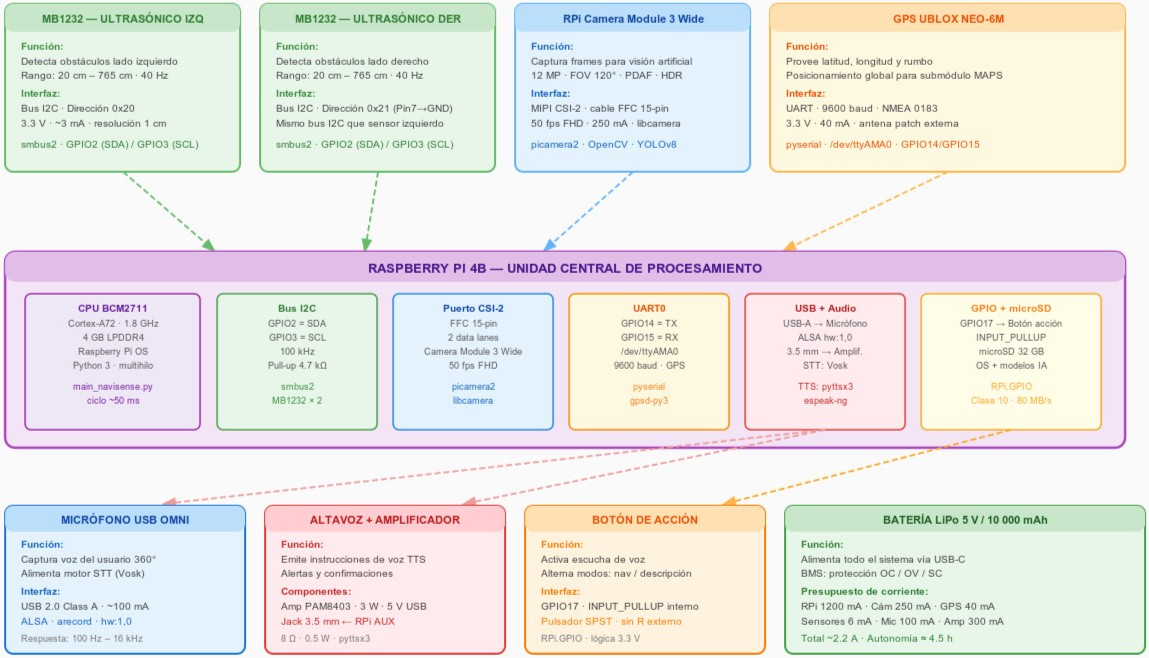
\includegraphics[width=0.8\textwidth]{Diagramas/electrosincables.jpg}
    \caption{Diagrama funcional de componentes electrónicos del sistema}
    \label{fig:bloques_electronica}
\end{figure}
 
La Figura~\ref{fig:conexiones_electronica} muestra el esquemático de conexiones
físicas del prototipo, donde se detallan los pines específicos de la Raspberry Pi
implicados en cada interfaz.
 
\begin{figure}[H]
    \centering
    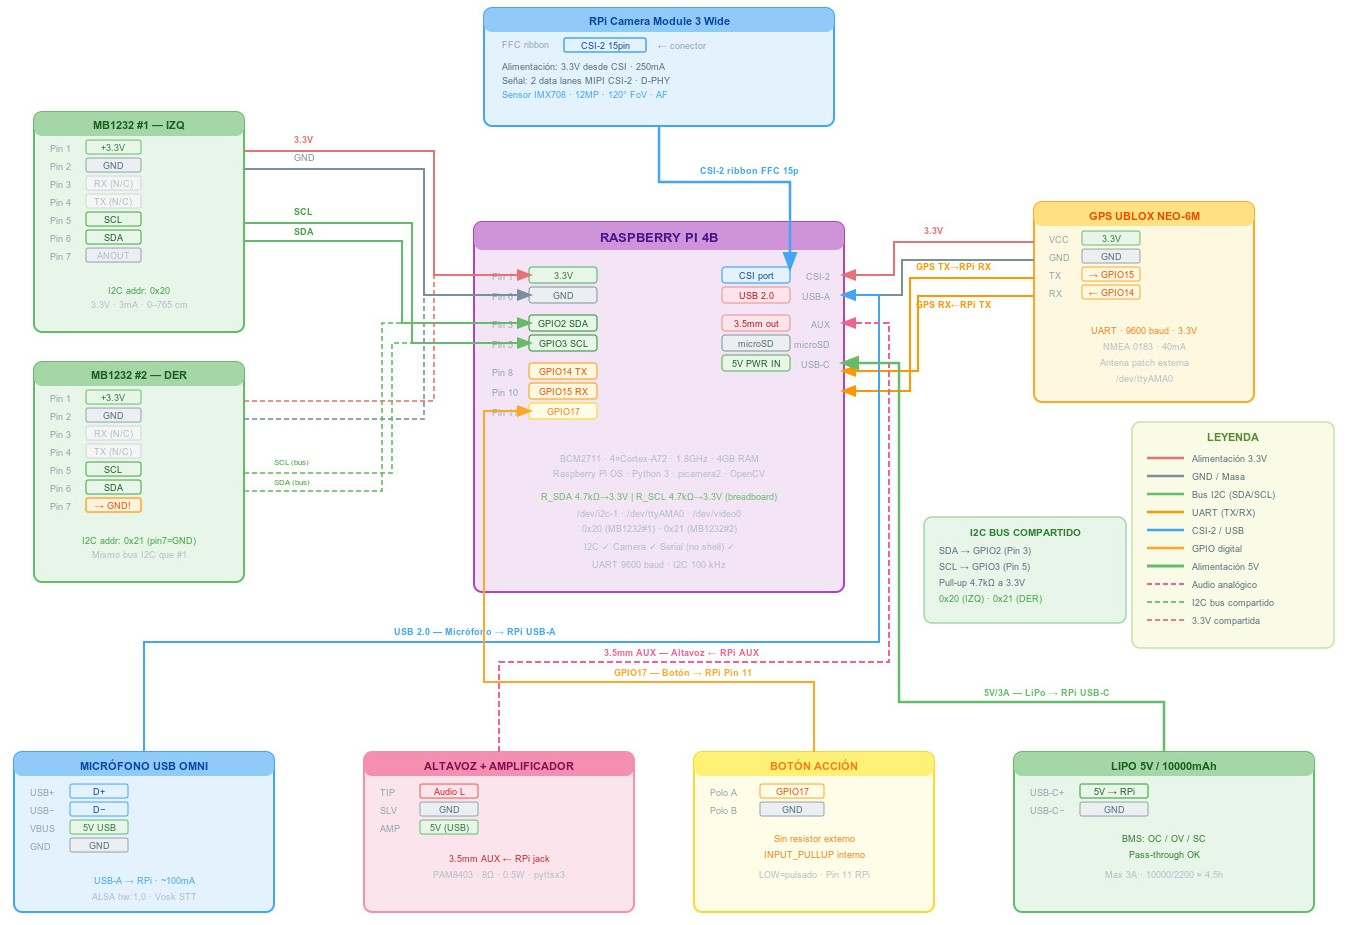
\includegraphics[width=0.88\textwidth]{Diagramas/electro.jpg}
    \caption{Esquemático de conexiones físicas del prototipo}
    \label{fig:conexiones_electronica}
\end{figure}

\subsection{Costos y viabilidad}

El sistema está diseñado para ejecutarse sobre hardware embebido de bajo costo,
siguiendo las restricciones establecidas en RNF-05 y RNF-10. La plataforma principal
es una Raspberry Pi, la cual ofrece la capacidad de procesamiento suficiente para
ejecutar la mayoría de los módulos del sistema bajo las latencias definidas en los
requerimientos. Sin embargo, debido a que algunas tareas como visión por computadora
o modelos de inteligencia artificial pueden demandar mayor capacidad de cómputo,
durante las pruebas se evaluará el desempeño general del sistema. En caso de detectar
limitaciones de rendimiento, se utilizará la conectividad Wi-Fi integrada de la
Raspberry Pi para establecer comunicación con una computadora personal que funcionará
como servidor de procesamiento, permitiendo ejecutar las tareas más pesadas de manera
remota sin modificar el funcionamiento general del sistema.

Para la percepción visual se selecciona el \textbf{Raspberry Pi Camera Module 3}, que
incorpora el sensor Sony IMX708 de 12~MP con tecnología CMOS \textit{back-illuminated
stacked}. Este módulo ofrece una buena calidad de imagen y resulta especialmente útil
en aplicaciones de visión por computadora debido a su sistema de autoenfoque y su
capacidad HDR, que ayudan a mantener imágenes más claras en diferentes condiciones
de iluminación, como cambios entre interiores y exteriores
\cite{raspberrypi_camera_doc3}. La versión Wide, con un campo de visión diagonal de
120°, permite capturar una mayor parte del entorno alrededor del usuario, lo cual es
ventajoso para navegación asistida y detección de obstáculos laterales. Además, su
compatibilidad nativa con Raspberry Pi y la biblioteca \texttt{libcamera} facilita
su integración con el sistema de procesamiento de imágenes
\cite{raspberrypi_camera_doc3}.

Para la detección de proximidad se utilizan \textbf{dos sensores MB1232}, colocados
en el frente del dispositivo, uno sobre cada cristal y apuntando en la misma dirección
que la cámara. Estos sensores fueron seleccionados debido
a que ofrecen lecturas más estables y confiables que alternativas más básicas como
el HC-SR04, especialmente en entornos urbanos donde puede existir ruido acústico o
eléctrico \cite{mb1232_datasheet}. Ambos sensores comparten el bus I2C de la
Raspberry Pi mediante la biblioteca \texttt{smbus2}, permitiendo una integración
compacta y sencilla. El MB1232 tiene un haz angosto, por lo que no es adecuado para
cubrir los costados; al frente, su haz coincide con lo que ve la cámara y permite
confirmar o descartar las detecciones visuales y detectar superficies que la visión no
reconoce, como vidrios y mamparas. La descripción de este montaje y su efecto en el
software se presenta en la Sección~\ref{sec:dev_prototipo}.

El sistema incorpora además un \textbf{botón para hablar}, que permite al usuario
activar o reiniciar la navegación sin depender completamente del reconocimiento de
voz. Esto resulta útil en ambientes con demasiado ruido o en situaciones donde el
usuario necesite interactuar rápidamente con el sistema.

La Tabla~\ref{tabla_hardware} detalla los componentes de hardware seleccionados para
el prototipo, junto con su función dentro del sistema, sus características principales
y su costo aproximado.

\begin{longtable}{p{4.2cm} p{4.5cm} p{2.8cm} p{1.8cm}}
\caption{Componentes de hardware del prototipo con costo aproximado}
\label{tabla_hardware} \\
\hline
\textbf{Componente} & \textbf{Función en el sistema}
    & \textbf{Especificación clave} & \textbf{Costo aprox.} \\
\hline
Raspberry Pi 4 Model B (4~GB RAM)
    & Unidad de procesamiento central. Ejecuta todos los módulos de software del sistema.
    & CPU quad-core Cortex-A72, 4~GB LPDDR4
    & \$75 USD \\
\hline
Raspberry Pi Camera Module 3 Wide (IMX708)
    & Captura continua de fotogramas para los módulos de percepción visual.
    & 12~MP, PDAF, HDR, FOV 120°, 50~fps FHD, CSI-2
    & \$25 USD \\
\hline
Sensor MB1232 I2CXL-MaxSonar (izquierda)
    & Medición de distancia al frente, sobre el cristal izquierdo. Dirección I2C
    \texttt{0x20}.
    & Rango 20~cm--765~cm, 1~cm res., I2C, 40~Hz
    & \$30 USD \\
\hline
Sensor MB1232 I2CXL-MaxSonar (derecha)
    & Medición de distancia al frente, sobre el cristal derecho. Dirección I2C
    \texttt{0x21}.
    & Rango 20~cm--765~cm, 1~cm res., I2C, 40~Hz
    & \$30 USD \\
\hline
Micrófono USB omnidireccional
    & Captura de audio para el módulo de reconocimiento de voz.
    & Respuesta 100~Hz -- 16~kHz, UAC class
    & \$15 USD \\
\hline
Altavoz + amplificador PAM8403 (3.5~mm)
    & Reproducción de instrucciones sintetizadas por el módulo de salida.
    & 8~$\Omega$, 0.5~W, conector AUX
    & \$10 USD \\
\hline
IMU de 9 ejes BNO055
    & Odometría del SLAM: orientación absoluta (giro) y aceleración lineal (conteo de
      pasos); inclinación de la cámara.
    & I2C \texttt{0x28}, fusión a bordo NDOF
    & \$35 USD \\
\hline
Botón de acción momentáneo
    & Activación o reinicio de sesión de navegación por hardware (GPIO17, pull-up interno).
    & SPST, lógica 3.3~V
    & \$2 USD \\
\hline
Batería LiPo 5~V 10000~mAh + BMS
    & Alimentación portátil del sistema completo vía USB-C. BMS con protección OC/OV/SC.
    & Corriente de salida máx. 3~A, pass-through
    & \$25 USD \\
\hline
Tarjeta microSD (32~GB, clase 10)
    & Almacenamiento del sistema operativo y modelos de IA.
    & Velocidad mínima 80~MB/s
    & \$10 USD \\
\hline
Resistencias pull-up 4.7~k$\Omega$ (×2)
    & Estabilización del bus I2C en líneas SDA y SCL.
    & 3.3~V, tolerancia 1\%
    & \$1 USD \\
\hline
\textbf{Total estimado} & & & \textbf{\$258 USD} \\
\hline
\end{longtable}
La estimación de costo total del prototipo es de aproximadamente \$258 USD, lo que lo
sitúa en un rango accesible para un prototipo de investigación de asistencia tecnológica.
El componente con mayor impacto en el costo son los sensores MB1232, cuyo precio unitario
supera al de los sensores ultrasónicos básicos, pero que se justifica por sus capacidades
de rechazo de ruido y calibración automática en tiempo real, necesarias para operar con
confiabilidad en los entornos ruidosos que describe la restricción RNF-06
\cite{mb1232_datasheet}. Los precios son estimaciones basadas en componentes disponibles
comercialmente y pueden variar según el proveedor y la región.